\documentclass[11pt]{article}
\usepackage{acl2016}
\usepackage{paralist}
\usepackage{subfig}
\usepackage{times}
\usepackage{latexsym}
\usepackage{graphicx}
\usepackage{url}
%\usepackage{subfigure}
\usepackage{pgfplotstable}
\usepackage{hyperref}
\usepackage{color}
\usepackage{lipsum,adjustbox}

\newcommand{\com}[1]{}
\newcommand{\secref}[1]{Section \ref{#1}}
\newcommand{\figref}[1]{Figure~\ref{#1}}
\newcommand{\tabref}[1]{Table~\ref{#1}}
\newcommand{\oa}[1]{\footnote{\color{red} #1}}
\newcommand{\bh}[2]{\footnote{\color{blue} #1}}

\newcommand\BibTeX{B{\sc ib}\TeX}


\title{HUME: Human UCCA-based Machine-Translation Evaluation}

\author{Author 1\\
	    XYZ Company\\
	    111 Anywhere Street\\
	    Mytown, NY 10000, USA\\
	    {\tt author1@xyz.org}
	  \And
	Author 2\\
  	ABC University\\
  	900 Main Street\\
  	Ourcity, PQ, Canada A1A 1T2\\
  {\tt author2@abc.ca}}

\date{}

\begin{document}

\maketitle

\begin{abstract}
  
  Recent interest in semantics-aware MT systems underscores the importance of
  semantic evaluation for Machine Translation (MT) systems. 
  A semantic measure, sensitive to possible semantic discrepencies
  between the translation output and the source, is likely support the construction
  and tuning of structure-aware MT, much in the same way that string-based measures,
  such as BLEU, enabled progress in shallower MT.
  We present a novel human semantic evaluation measure for MT, Human
  UCCA-based MT evaluation (HUME), building on the UCCA semantic representation scheme.
  Making progress over previous work, the proposed measure takes into account
  a wider range of semantic phenomena and does not rely on semantic annotation
  of the MT output itself, whose interpretation is often unclear.
  We experiment with four language pairs, demonstrating HUME's broad applicability,
  as well as its reliability, reflected in its inter-annotator agreement rates.

\end{abstract}


%%%%%%%%%%%%%%%%%%%%%%%%%%%%%%%%%%%%%%%%%%%%%%%%%%%%%%%%%%%%%%%%%%%%%%%%%%%%%%%%%%%%%%
\section{Introduction}\label{sec:intro}

Human judgement is the central, and perhaps most fundamental, criterion for
estimating the quality of an MT system.
Nevertheless, common measures for MT evaluation, such as adequacy and fluency judgements
or the relative ranking of several possible translations, are problematic in two ways.
First, as the quality of translation is determined by multiple factors, it is difficult
to assign a single number that quantifies the quality of the entire sentence. This
is indeed reflected in the diminishing inter-annotator agreement rates of human ranking measures
as a function of the sentence length \cite{Bojar:2011}.
Second, a sentence-level quality score does not indicate what parts of the sentence
are erroneously translated, and hence cannot inform developers in overcoming these errors.

These problems were partially addressed by measures that decompose over sub-parts of the evaluated
translation sentence (henceforth, {\it translation}),
most commonly over its words or n-grams,
quantifying the overlap of its sub-parts relative a reference translation.
More recent work on MT evaluation proposed measures
that decompose over semantically defined units,
quantifying the similarity of the output and the reference in terms of
their verb argument structure (the most notable of these measures is
MEANT \cite{lo2011structured}).
While allowing to localize semantic errors in the translation,
these measures' focus on verb argument structures misses out on many pervasive semantic phenomena,
such as inter-clause linkage and nominal argument structures, and thus only provides
a limited perspective on the semantic similarity between the output and reference.
Moreover, assigning semantic structure to MT output, especially when low in quality,
is difficult and arguably ill-defined.

We propose the Human UCCA-based MT Evaluation ({\it HUME}) metric,
a human evaluation measure that decomposes over the semantic units of the sentence.
Semantic units are defined according to the 
UCCA scheme \cite{abend2013universal}, an appealing candidate for semantic analysis,
due to its cross-linguistic applicability, support for rapid annotation, and coverage
of many fundamental semantic phenomena, such as verbal, nominal and adjectival
argument structures and the inter-relations between them.

HUME operates by aggregating human assessments of the translation quality of individual
semantic units in the source sentence.
Importantly, HUME only requires semantically annotating the source sentence,
thus avoiding the annotatation of machine-generated text 
and allowing re-use of the source semantic annotation for measuring the quality
of different translations of the same source sentence.
By basing the measure on a direct comparison
of the source and translation we avoid the difficulties engendered by using
reference translations, albeit at the cost of imposing the additional requirement
that the evaluator be proficient in both the source and target languages.
See \secref{sec:hmeant_comp}.

We conduct experiments with four language pairs: English-German, English-Polish,
English-Romanian and English-Czech, and report efficiency (time of annotation) and
inter-annotator agreement scores, as well as qualitative comparison of the resulting
HUME scores with crowd-sourced adequacy judgements. Results show that HUME obtains 
agreement scores which are on par with those of standard sentence-level ranking measures,
but unlike them, HUME's scores do not decrease with logner sentences.
The paper concludes by outlining ongoing work to construct semi- and
fully-automatic variants of HUME.


%%%%%%%%%%%%%%%%%%%%%%%%%%%%%%%%%%%%%%%%%%%%%%%%%%%%%%%%%%%%%%%%%%%%%%%%%%%%%%%%%%%
\section{Background}\label{sec:background}

%While the measure addresses the two major shortcomings 
%detailed above, it is unable to capture semantic differences which do not show up in 
%the verb-argument structure, including several very frequent phenomena, 
%Another shortcoming of MEANT is its reliance on semantically annotating MT output,
%which is often unintelligible. Finally, measures based on a comparison to a


%These difficulties have motivated the definition of a human measure that decomposes over
%the semantic structure of the sentence, rather than its n-grams. The most notable attempt of
%this type is the MEANT measure, and its human variant HMEANT
%\cite{lo2010evaluating,lo2011structured,Lo2011meant,lo2013meant}, which quantifies the
%similarity between the output translation and a reference translation in terms of the similarity
%between their verbal argument structures
%While the measure addresses the two major shortcomings
%detailed above, it is unable to capture semantic differences which do not show up in
%the verb-argument structure, including several very frequent phenomena, such as
%inter-clause linkage, nominalizations and copula clauses
%(see \secref{sec:hmeant_comp}).
%Another shortcoming of MEANT is its reliance on semantically annotating MT output,
%which is often unintelligible. Finally, measures based on a comparison to a
%reference translation
%are necessarily incomplete, as they compare to a small number of references
%out of the the huge number of possible translations a sentence may have
%\cite{dreyer2012hyter}.


\paragraph{Machine Translation Evaluation.}
%MT evaluation has been traditionally pursued through human-based
%evaluation that quantifies the adequacy of the translation in preserving the meaning 
%of the source sentence, and its fluency as a sentence in the target language \cite{lopez2008statistical}.
Human evaluation is generally determined
either according to the relative ranking of the outputs of multiple systems
e.g., in the WMT shared tasks \cite{bojar2015findings}, or by assigning
indiviaul adequacy/fluency scores to each translation, a procedure recently improved
by \newcite{graham2015improving}.
However, while providing the gold standard for MT evaluation, human evaluation is not a scalable solution,
and is unfeasible where a wide variety of systems or parameter settings are to be evaluated.
% has motivated the construction of cheaper methods that correlate with human
%judgement.

Scalability is addressed by employing automatic and semi-automatic approximations of human
judgements. Most commonly, such scores decompose over the sub-parts of
the translation, and quantify how many of these sub-parts appear in a reference translation,
whose validity has been manually confirmed. This decomposition further allows system developers
to localize the errors within the translation.
The most commonly used measures decompose over n-grams or even individual words, e.g., 
the BLEU \cite{Papineni:2002}, NIST \cite{Doddington:2002} and METEOR measures \cite{Banerjee:2005}.
Another common approach is to determine the similarity between the reference and translation
by applying string edit distance \cite{snover2006study}.
While these measures stimulated much progress in MT research by allowing
the evaluation of massive-scale experiments,
their decomposition over words and n-grams is better suited for localizing errors
in the output of shallow MT methods, and is less instructive in identifying the semantic
nature of the errors. 

%These methods are most suitable for evaluating shallow MT approaches and are
%less instructive as to what aspects of the reference's meaning were not preserved
%in the translation output.
%A common approach is to compare the MT output with reference translations,
%created or verified by an expert. Methods often rely on some sort of string matching
%methods, such as overlap of n-grams, as with the BLEU and METEOR measures, or edit
%distance.
%First, they rely on comparison to reference translations, which reflect a small
%number out of the enormous number of ways to translate a sentence and are thus
%inherently incomplete. 

In order to address this shortcoming, more recent work quantified
the similarity of the reference and translation in terms
of their {\it semantic structure}. \newcite{liu2005syntactic} took a syntactic approach, 
quantifying the similarity between the syntactic structures of the reference and translation.
\newcite{owczarzak2007evaluating} took a similar approach using lexical-functional grammar structures.
\newcite{gimenez2007linguistic} proposed to aggregate multiple types of information,
capturing the overlap between the output and reference in terms of their
semantic (predicate-argument structures), lexical and morphosyntactic features.

Perhaps the most notable attempt at semantic MT evaluation is MEANT and
its human variant HMEANT, which quantifies the similarity between
the reference and translation in terms of the overlap in
their verbal argument structures structures, and associated semantic roles.
We discuss the differences between HMEANT and HUME in \secref{sec:hmeant_comp}.

\begin{figure}
  
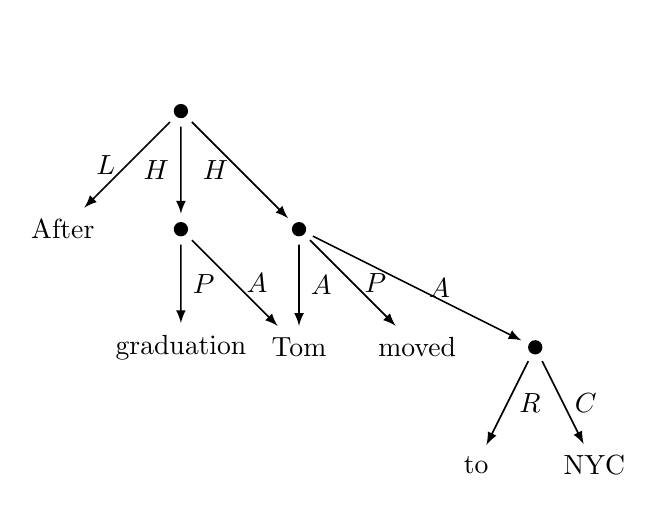
\begin{tikzpicture}[semithick, x=2.4cm,y=0.8cm, >=latex, baseline=7ex,
      inner sep=.3ex, outer sep=.7ex, minimum size=1.2ex,->]
    \node (ROOT) [fill=black, circle] {}
    child {node {After} edge from parent node[left]  {$L$\hspace{1.5cm}}}
    child {node (H1) [fill=black,circle] {}
      child {node {graduation} edge from parent node[right] {$P$}}
      %child {node {to Paris} edge from parent node[right] {$A$}}
      edge from parent node[left] {$H$}
    }
    child {node (H2) [fill=black,circle] {}
      child {node {} edge from parent[draw=none]}
      child {node {} edge from parent[draw=none]}
      child {node (Tom) {Tom} edge from parent node[right] {$A$}}
      child {node {moved} edge from parent node[right] {$P$}}
      child {node [fill=black,circle] {}
        child {node {to} edge from parent node[right] {$R$}}
        child {node {NYC} edge from parent node[right] {$C$}}
        edge from parent node[right] {$A$}}
      %child {node {to Paris} edge from parent node[right] {$A$}}
      edge from parent node[left] {$H$}
    };
    \draw (H1) -> (Tom) node[midway, right] {$A$ \hspace{0.2cm}};
  \end{tikzpicture}
\caption{\label{fig:ucca_example}
  Sample UCCA annotation.}
\end{figure}


\paragraph{Semantic Representation.}
UCCA (Universal Conceptual Cognitive Annotation) is a cross-linguistically applicable, lightweight
scheme for semantic annotation. Formally, a UCCA structure is a directed acyclic graph (DAG),
whose leaves correspond to the words of the text.
The graph’s nodes, called {\sc units}, are either terminals or several elements jointly
viewed as a single entity according to some semantic or cognitive consideration. Edges bear
a category, indicating the role of the sub-unit in the relation the unit represents. UCCA
currently focuses on annotating argument structures (adjectival, nominal, verbal and others) and
relations between them. The most basic notion is the {\sc scene}, which describes a movement, an
action or a state which is persistent in time. Each Scene contains one main relation, as well
as one or more participants. For example, the sentence ``After graduating, Tom moved to NYC''
contains two Scenes, whose main relations are ``graduating'' and ``John''. The participant ``John''
is a part of both Scenes, while ``NYC'' only of the latter. Further categories account for
relations between Scenes and the internal structures of complex participants and relations.
See \figref{fig:ucca_example}.

% UCCA Motivation
UCCA is a natural candidate for defining a semantic
MT evaluation measure for a number of reasons. 
First, it defines a coarse-grained and intuitive set of categories,
and consequently can be reliably annotated by non-experts, after as little as two hours
of training \cite{marinotti2014}.
Second, UCCA is a cross-linguistically applicable scheme, seeking to represent what is shared between languages,
by building on linguistic typological theory, and specifically on ``Basic Linguistic Theory''
\cite{Dixon:10a,Dixon:10b,Dixon:12}, one of the most widely used frameworks for linguistic description.
Indeed, UCCA's cross-linguistic applicability has been demonstrated through its
application to annotation in English, French, German and Czech\oa{Did we do experiments on Czech?}. 
Third, the scheme has been shown to be semantically stable
in translation: UCCA annotations of translated text usually contain the same set of relationships
\cite{sulem2015conceptual}. This is an indication that the scheme reflects
a common layer of representation that in a correct translation
is mostly shared between the translation and the source. 
We note that that verbal argument structures are less stable in this sense, as a verbal
argument structure may be translated or paraphrased to a nominal or adjectival
argument structure, and are thus less suitable as a basis for a semantic measure.
For example, ``after he graduated, Tom moved to NYC''
conveys a similar meaning to ``after graduation, Tom moved to NYC''. 

While most broad-coverage semantic work focused on shallow semantic structures,
predominantly argument structures annotated with their semantic roles, much recent
interest has been devoted to defining more complete semantic representation schemes.
The Abstract Meaning Representation (AMR) scheme \cite{banarescu2013abstract}
shares much of UCCA's motivation for defining a more complete semantic annotation.
However, using AMR is not optimal for defining a decomposition of a sentence into semantic
units as it does not ground its semantic symbols in the text,
thus not straightwardly allowing a decomposition of the sentence into sub-units.
Moreover, AMR is more fine-grained than UCCA and consequently more difficult to annotate.\oa{should we
  add that it is less cross-linguistically stable? maybe that's an overkill..}

Other approaches have been proposed for semantic representation, which are grounded in the words
and phrases of the text, and have generally represented semantic structures as bi-lexical dependencies.
Examples include the Prague Treebank tectogrammatical layer \cite{hajic2012announcing}, as well
as dependencies derived from Minimal Recursion Semantics representations \cite{oepen2006discriminant}.
Nevertheless, despite their appeal as deep and intuitive means for semantic representation,
these approaches require linguistic expertise for their annotatation, due to the intricate and
fine-grained distinctions they provide, and are thus in our view less suitable for basing
an interpretable MT evaluation on. 
%\newcite{Basile:12} attempted to make some aspects of the semantic annotation more accessible,
%but to our knowledge no results of this brand have been reported.


%%%%%%%%%%%%%%%%%%%%%%%%%%%%%%%%%%%%%%%%%%%%%%%%%%%%%%%%%%%%%%%%%%%%%%%%%%%%%%%%%%%
\section{The HUME Measure}\label{sec:hume}

%We do not distinguish fluency and adequacy judgements, as they are correlated anyway \cite{ccb}.


\subsection{Annotation Guidelines}\label{sec:guidelines}
In this section we summarise the procedure for annotating machine translation output.

There are two manual steps in the annotation process. The first is to create UCCA annotations for the source sentence,
following the
UCCA guidelines\footnote{All UCCA-related resources can be found here: \url{http://www.cs.huji.ac.il/~oabend/ucca.html}}. Source sentences are all in English, and the annotation was performed by four
computational linguists\oa{were there no other annotators from Prague?}. After we have the UCCA annotation on 
the source, we use the word-to-word alignments from the MT system in order to project this annotation to the MT output,
and use native speakers of the target language in order to annotate this output. Since these annotators have to
judge the quality of the translation, they also needed to be fluent in English.\bh{Somewhere we could explain that we
could do a similar annotation with monolinguals, although it entails aligning reference and MT output}

The basic strategy for annotating HUME on the  MT output to step through the source sentence semantic 
components (projected UCCA nodes), looking at the translation via the word alignments, and marking
on the source structure which parts have been correctly translated.
There are two kinds of components (nodes): a word or basic semantic unit, and a structural component
which contains one or more sub-components. 

\paragraph{Lexical nodes} are usually comprised of individual words. They are the leaf nodes of the tree,
the smallest meaning-bearing units.
Leaf nodes can be labelled as green (correct), orange (partially correct) and red (incorrect). 
The traffic light system makes the marking of the
lexical units as simple as possible.

\begin{compactdesc}
\item[Green] The meaning of the word or phrase has been largely captured.
\item[Orange] the essential meaning has been captured, but some part of the translation is wrong. 
For example, this could often be due to the translated word having the wrong tense, or the wrong morphology. 
\item[Red] The essential meaning of the unit has not been captured.
\end{compactdesc}


\paragraph{Structural nodes} contain other nodes which could be either lexical or structural nodes, 
and they can be labelled as ``Adequate'' or ``Bad''. 
What we are trying to gauge for structural nodes
is if the children of these nodes
relate to each other in the same way in the source sentence and in the translation. 
There are many ways that the relationship between the children might go wrong in translation:
\begin{compactitem}
\item One of the child nodes is missing from the aligned translation. 
\item An extra word or phrase has been inserted into the aligned  translation.
\item The components of the translation are ordered differently 
%to 
from
the source.
\end{compactitem}

If any of these changes have occurred and this damages the meaning of the aligned translation, then we mark the 
structural node as ``Bad''. 
However if the arrangement of the child nodes is essentially correct, except that one or
more of the child nodes has themselves been translated wrongly (and so is marked
orange or red), then the structural node should be 
annotated as ``Acceptable''.

\begin{figure*}[t]
    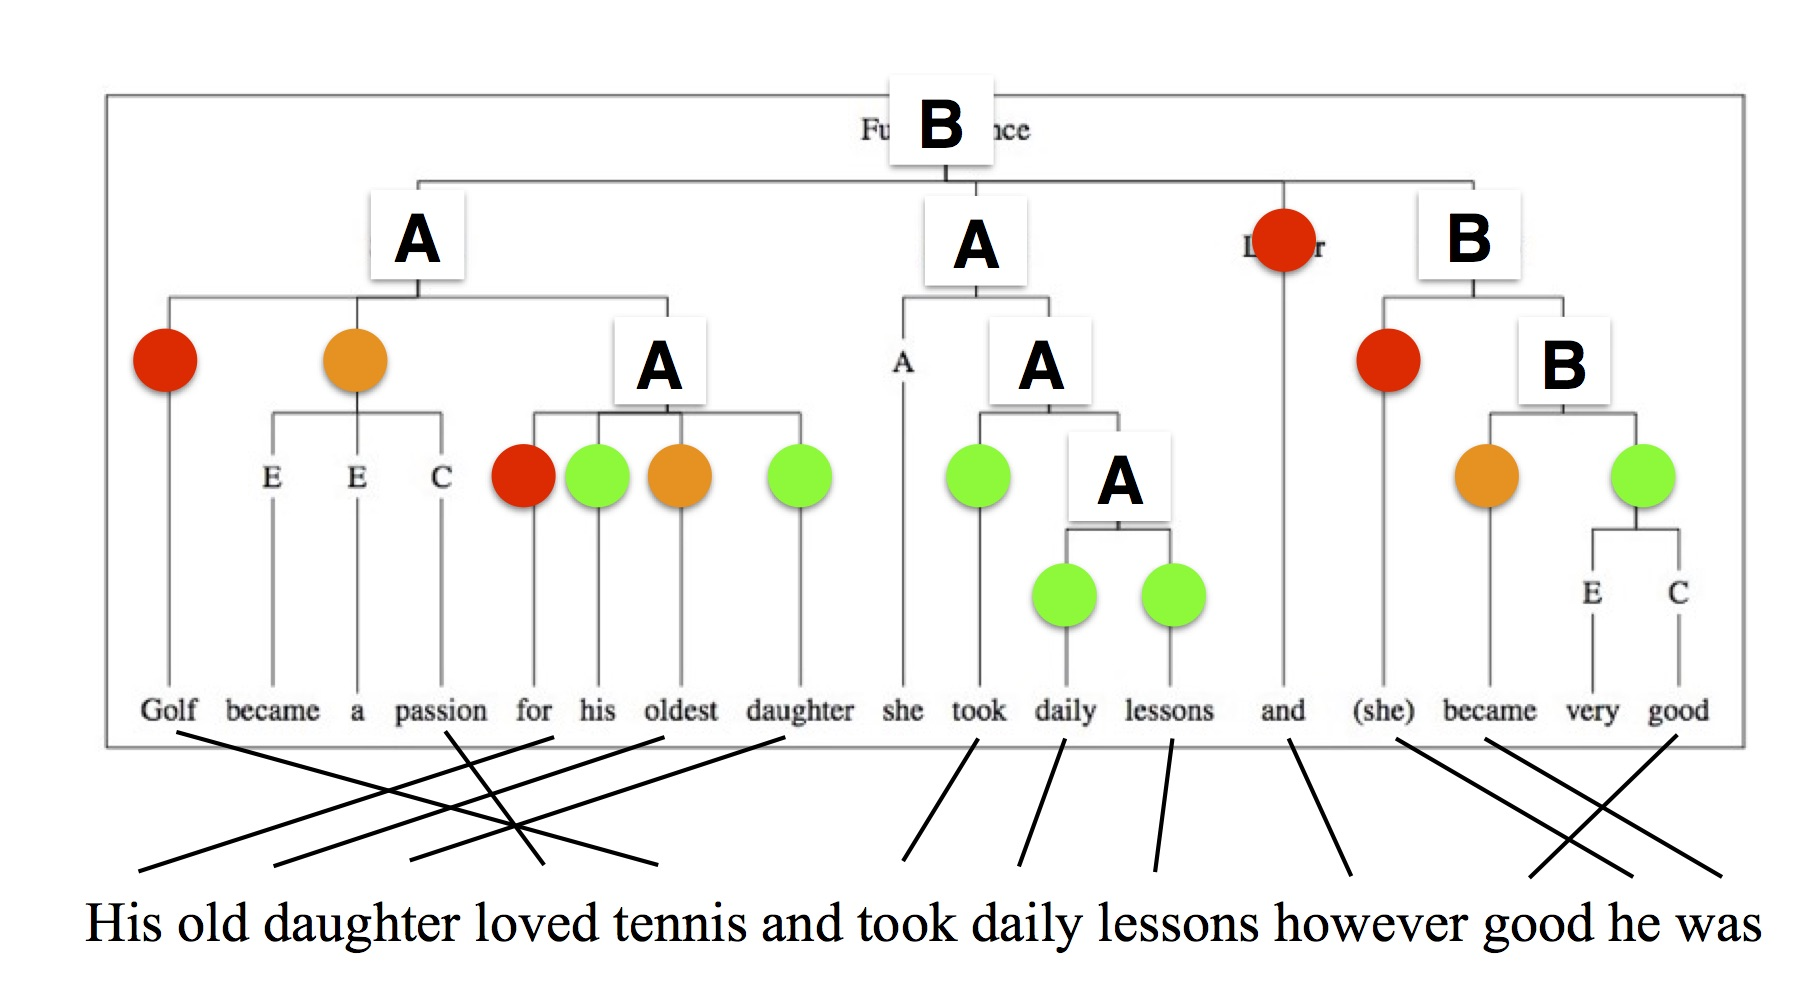
\includegraphics[width=1\textwidth]{ucca-tree-mteval}
    \caption{UCCA Tree evaluated in comparison to an aligned ``translation'' (an
	English paraphrase).}
    \label{ucca-tree-mteval}
\end{figure*}

%TODO describe figure 2 here

There are cases where we cannot usefully compare individual words in the source to words in the target.
We often need to compare translation at the phrase level. If this is the case, then we can 
 treat the structural node as a lexical unit, and mark it with the traffic light labels. This 
means that none of the children of this node will be examined in order determine the semantic score
for this sentence. 
In Figure~\ref{ucca-tree-mteval}, we can see that the phrase ``became a passion'' has been labelled as a lexical
node and it has been evaluated as ``Orange'', or partially correct, as the translation of this phrase ``loved'' 
only partially capture the semantics of the source.

We are separating lexical and structural evaluation in order to simplify evaluation and to localise errors
to their point of origin. For this reason, if a word has been translated incorrectly,
the parent node should still be correct if the number and relationship between its children are the same
as in the source. 
In Figure~\ref{ucca-tree-mteval}, we can see that even though an important child of the first scene is 
incorrectly translated (``Golf''), and the children of are ordered differently, 
the scene itself is marked as ``Acceptable''. The translation of the scene retains the structural 
relationships between the children.
\\

\begin{figure*}[t]
    \begin{center}
    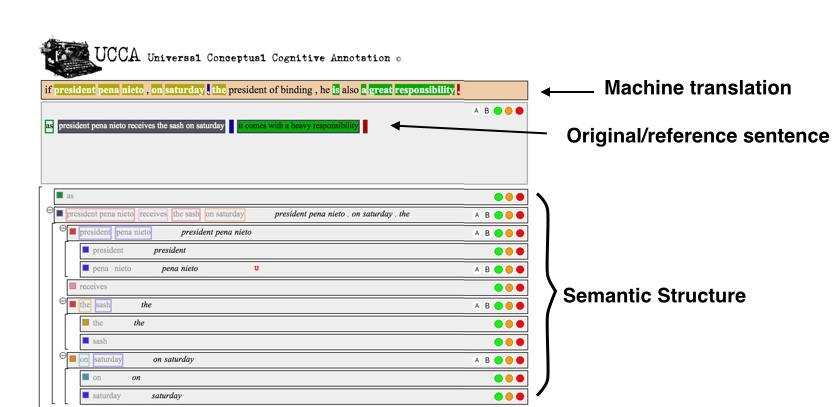
\includegraphics[width=1\textwidth]{interface-annotations}
    \caption{The HUME annotation tool, based on the UCCA tool}
    \label{mttool}
    \end{center}
\end{figure*}

In Figure~\ref{mttool} you we show the MT evaluation tool. The sentence at the top shows the complete MT system output. Underneath the MT output is the  source sentence.  Underneath the source sentence we see its expandable semantic tree structure with both lexical and structural nodes. Lexical nodes only have traffic light annotation, whereas a structural node would normally be labelled ``A'' or ``B'' but could also be labelled as a lexical node, in the case where there is no word to word correspondence for the translation of its children.

 The child components of a structural node are marked with different coloured rectangles. When navigating through the different source sentence nodes, one can see the relevant sections of the translation because the aligned words in the translation are highlighted in the complete sentence above. Aligned translations are also shown in black alongside the source node. If the node is aligned to a set of discontiguous words in the translation, then the unaligned words that appear in between the aligned words are shown in red. Even if these words are not directly aligned to the source node, they 
will likely change the meaning of the translation and must be considered when marking 
the translation as correct or not. The alignments are meant just as a guide. The annotator should  look at the complete translation when deciding on the evaluation of a node. The translation could have content added before or after the node which changes its
 structure or meaning. If an extra component is prepended to a structural node, for example, it should be marked as ``Bad''.



\subsection{Composite Score}\label{sec:score}

composite score (uniform, sub-sets, weighted rather not -- according to categories [or empirically according to agreement])


\subsection{Comparison with HMEANT}\label{sec:hmeant_comp}

HMEANT shares much of HUME's motivation for providing a
measure that decomposes over semantic units, rather than strings, but focuses on verbal
argument structures, ignoring other pervasive phenomena such as nominal predicates, inter-clause
relations and copula clauses.
HUME further diverges from both MEANT and the shallower BLEU and
METEOR measures, in not requiring a reference.
Instead, it compares the source directly with the output
translation. We see this difference as crucial where semantic analysis is concerned, as it
is often impossible to assign a semantic structure to a low quality MT output sentence.
See \secref{sec:hmeant_comp} for a more elaborate discussion of the differences between HUME
and HMEANT.


For instance, consider the sentence ``A coronary angioplasty may not be technically possible'',
which was translated by one of the systems we experimented with as
``Eine koronare Angioplastie kann nicht technisch m{\"o}glich'', i.e., the main verb ``sein'' (``be'') is omitted.
While this may be interpreted is a minor error, HMEANT will assign it a very low score, as it failed to
translate the main verb. 

We conducted an analysis of the English UCCA Wikipedia
corpus, comprising
of 5324 sentences,
in order to assess the frequency of some of the major phenomena HMEANT fails to address,
Coppula cluases are treated in HMEANT simply as instances of the main verb ``be'', which
generally does not convey the meaning of these clauses. They appear in 21.7\% of the sentences,
according to a conservative estimates that only considers non-auxilliary instances of ``be''.
Nominative argument structures, which are completely ignored under HMEANT are in fact highly
pervasive, appearing in 48.7\% of the sentences. Linkers expressing an inter-relation between
clauses (mainly discourse markers and coordinating conjunctions) appear in 56\% of the
sentences\footnote{Argument structures and linkers are explicitly marked in UCCA. We identified
  non-auxilliary instances of ``be'' and nouns using the NLTK standard tagger.}.
We are not aware of any empirical evaluation that demonstrates that verb argument structure,
taken alone, capture the crux of the sentence semantics meanings, and so the coverage of
further phenomena by HUME will first allow to determine empirically
(rather than stipulate), what semantic structures are important
to preserve for MT translation, and which are less important




%%%%%%%%%%%%%%%%%%%%%%%%%%%%%%%%%%%%%%%%%%%%%%%%%%%%%%%%%%%%%%%%%%%%%%%%%%%%%%%%%%%
\section{Experiments}\label{sec:experiments}

In order to validate the HUME metric, we ran an annotation experiment with one source language (English), and four 
target languages (Czech, German, Polish and Romanian), using text from the public health domain. We are 
particularly interested in this domain since our ultimate goal is to provide high-quality translations of health
information for speakers of languages other than English, and in this domain accurate transfer of meaning is
paramount.

Our annotation experiment sought to address the following questions:
\begin{itemize}
\item Can HUME be annotated quickly and reliably, and does the reliability still hold for longer sentences.
\item Can HUME capture translation issues that other annotation schemes (such as adequacy judgements and HMEANT
cannot)?
\item What can HUME annotation tell us about the strengths and weaknesses of MT?
\end{itemize}

\bh{Maybe we should remove the third one, we
probably don't address it in this paper}

\subsection{Data Sets and Translation Systems}

For each of the four language pairs under consideration  we built phrase-based MT systems
using Moses \cite{Koehn:2007}. We used large training sets extracted from OPUS \cite{tiedemann:2009}, and
the data sets released for the WMT14 medical translation task \cite{bojar-EtAl:2014:W14-33}, to provide between
45 and 85 million sentences of training data, depending on language pair.

These translation systems were used to translate texts derived from both NHS 24\footnote{\url{http://www.nhs24.com/}} and 
Cochrane\footnote{\url{http://www.cochrane.org/}} into the four languages. The first organisation is a public body
providing healthcare and health-service related information in Scotland, whereas the second is an international NGO which 
provides independent systematic reviews on health-related research. From NHS 24, we selected the segments from their
``Health A-Z'' which is part of the NHS Inform website, and the Cochrane texts come from their plain language summaries
and abstracts.\bh{How much more do we need? Perhaps in the intro we could justify our focus on public health text
(accuracy!). The test corpora should have a public URL by the time we submit, although of course the source texts were 
already public anyway, and Lexi did some selection of examples for use in this expt. -- do we have to explain this?}

\subsection{Annotation Statistics}

For the annotation of MT output, we recruited seven annotators, two for each of the target languages apart from Czech. They were
all native speakers of the target languages and fluent in English. For Czech, we also recruited a  group of additional annotators
to annotate small numbers of sentences each for the purpose of calculating inter-annotator agreement. In \tabref{tab:annot}
we show the total number of sentences and nodes annotated by each annotator, where we consider the additional Czech
annotators as a single annotator. Note that not all nodes in all sentences were annotated. Sometimes this was because the
annotator did not finish a node, or accidentally missed a node, but in many cases it was also because it was an implicit 
UCCA node, which was not shown to the annotators since there is no corresponding source segment.
\begin{table}
\begin{center}
{\small
\begin{tabular}{ll|cccc}
& & cs & de & pl & ro \\
\hline
Sentences &  Annot. 1 & 324   & 339  & 351  & 230  \\
 & Annot. 2 & -- & 104  & 340  & 337 \\
\hline
Nodes & Annot. 1 & 8794  & 9253 & 9557  & 6152 \\
 &Annot. 2 & -- & 2906  & 9303  & 9228  \\
\end{tabular}
}
\caption{Total numbers of sentences and nodes annotated on the MT output.}
\label{tab:annot}
\end{center}
\end{table}

\emph{Timing of annotations}

\emph{Describe the UCCA annotation}

%\subsection{Data}\label{sec:data}

%\subsection{Efficiency of Annotation}\label{sec:efficiency}



\subsection{Inter-Annotator Agreement}
\label{sec:iaa}
\begin{itemize}
  \item Multiple annotation stats
  \item Kappas -- ROG, AB
  \item Kappa versus length
  \item Kappa versus bleu?
\end{itemize}

\oa{what is the purpose of the BLEU binning? is it because low quality and high
quality translations often diverge in their agreement scores?}



In order to assess the consistency of the annotation, we measure the Inter-Annotator
Agreement (IAA) using Cohen's Kappa on the multiply-annotated portions of the data.
For German, Polish and Romanian we used two annotators, so we report IAA on the overlap
between these annotators. For Czech we used one main annotator, plus several other extra
annotators to provide IAA. 

To calculate Kappa, we consider the annotation task as a classification task on 
nodes. We only consider nodes where there are at least two annotations from different
annotators and we treat nodes with more than two annotations as a set of paired
annotations\bh{This may not be correct, so should/could we do Kappa across the 
variable multiple annotations on Czech}. We consider Kappa separately on the lexical
nodes (annotated as red, orange or green) and the structural nodes (annotated
as acceptable or bad) since there should not be any confusion between these two types of
nodes. The small number of nodes which one annotator had labelled as structural and 
the other as lexical were ignored for the purposes of IAA, since such cases of annotator 
error could be caught by improved tool support.  The Kappas are shown in \tabref{tab:iaa}
\begin{table}[!ht]
\begin{center}
\begin{tabular}{l|cccc}
 & cs & de & pl & ro \\
\hline
Sentences & -- & 102 & 334 & 217 \\
\hline
Lexical nodes & -- & 1724 & 5386 & 3570 \\
Kappa & -- & 0.29 & 0.54 & 0.50 \\
\hline
Structural nodes & & 1040 & 2655 & 1989 \\
Kappa & -- & 0.44 & 0.33 & 0.58 \\
\end{tabular}
\caption{Inter-annotator agreement for the multiply-annotated portions of the data, as
measured by Cohen's Kappa. }
\label{tab:iaa}
\end{center}
\end{table}


To assess whether, as we hoped, HUME would make it easier to reliably annotate long sentences,
we binned the sentences according to length and measured Kappa on each of the bins. Each bin covers
a length range of 10, and we show the variance of kappa with length in \figref{fig:iaalength}.\bh{Note that cs is missing}

\def\iaafig #1{\includegraphics[width=7cm]{iaa_length_#1.png}}

\begin{figure*}[ht!]
\begin{tabular}{cc}


\subfloat[English-Czech]{
  \iaafig{de}
}
&
\subfloat[English-German]{
  \iaafig{de}

}
\\

\subfloat[English-Polish]{
  \iaafig{pl}
  
}
&
\subfloat[English-Romanian]{
  \iaafig{ro}

}
\end{tabular}
\caption{Inter-annotator Agreement (Kappa) versus sentence length, separately for
structural and lexical nodes. }
\label{fig:iaallength}


\end{figure*}


\subsection{Discussion of Disagreements}\label{sec:disagreements}


\subsection{Comparison with Crowdsourced Adequacy Judgements}\label{sec:adequacy}



%%%%%%%%%%%%%%%%%%%%%%%%%%%%%%%%%%%%%%%%%%%%%%%%%%%%%%%%%%%%%%%%%%%%%%%%%%%%%%%%%%%
\section{Conlusion}\label{sec:conclusion}










%%%%%%%%%%%%%%%%%%%%%%%%%%%%%%%%%%%%%%%%%%%%%%%%%%%%%%%%%%%%%%%%%%%%%%%%%%%%%%%%%%%
\section{Human Semantic Evaluation}

\oa{mention TER: using insertions, deletions, substitutions and shift of the entire sentence}

\label{sec:sem-eval:human}
We focus on producing high accuracy machine translation systems, but common 
automatic MT metrics are not able to directly capture accuracy. Even previously suggested methods
for using humans to evaluate accuracy are highly problematic. We aim to  develop a human evaluation method 
which is reliable and affordable and apply it to the MT prototypes. 
%This 
The
work described
in this section relates to 
%the 
task
\emph{T5.2: Human semantic evaluation}.
% defined in the description of action. 


In November 2015, we ran an evaluation task with 6 bilingual annotators, 2 from NHS 24 and 4 from Cochrane. 
We asked them to annotate about 350 sentences translated with the HimL year one systems 
and they had a budget of  up  to 40 hours each to perform this task. 
In this section we motivate and describe the experiment that we ran and we provide an initial analysis of
the results. In  Year 2 and Year 3 we will refine this evaluation task and use it to track the progress of our HimL prototypes.


\subsection{Overview}

Semantic evaluation of machine translation has typically been done at the sentence level and
we propose an  approach which breaks down the evaluation into basic semantic units, making evaluation 
simpler and more consistent. 
Our  assumption is that the semantic structure on the source sentence should be 
retained in the translation, and if it is not, then some essential part of the meaning 
%will be 
is
lost. 
The semantic framework that we base our evaluations on is called 
Universal Conceptual Cognitive Annotation \shortcite{abend2013universal}.  
UCCA has been developed using linguistic theories about 
what types of components and structures are universal across many different languages.

Our goal is to quantify how much of the meaning of the source sentence is preserved through translation.
There have been many approaches to evaluating the quality of machine translation, but most of them
have asked the annotator to give a score for the entire sentence. There are of course many ways 
that a translation can be incorrect and asking an annotator to provide a global score for a sentence
is a cognitively difficult task even if e.g. limited to a relative comparison
with another candidate translation. How serious is an error? What is the impact of multiple errors on global meaning?
By using UCCA structure to break the evaluation into meaningful components, we provide 
a more consistent and reliable method of evaluating translation accuracy.

The annotation proceeds as follows. Firstly, the source sentences (English, in our case) are annotated with UCCA trees. This
annotation is normally performed by computational linguists, and requires some training in UCCA, but the annotation can be 
reused for different target languages and different MT systems. 
We then create translations of the source sentences with the
MT system, collecting the word alignments from 
%
the
source sentence to 
the
translation provided by the system. These word
alignments are used to project the UCCA annotation from the source sentence to the the translation output, and then bilingual
annotators go through each projected UCCA node, assessing how well it is translated.  
We can estimate the impact of individual errors given their location in the semantic structure 
and we can thus extract a score for the whole sentence. More details on the procedure are provided 
below.


\subsection{Semantic Annotation}

The source sentences in this annotation scheme have been annotated with  a semantic structure defined as
Universal Conceptual Cognitive Annotation (UCCA).  UCCA was developed in the Computational Linguistics Lab of the Computer Science Department of the Hebrew University by Omri Abend and Ari Rappoport.
UCCA views the text as a collection of scenes (or events)
and their inter-relations and participants. 

\begin{figure*}[t]
    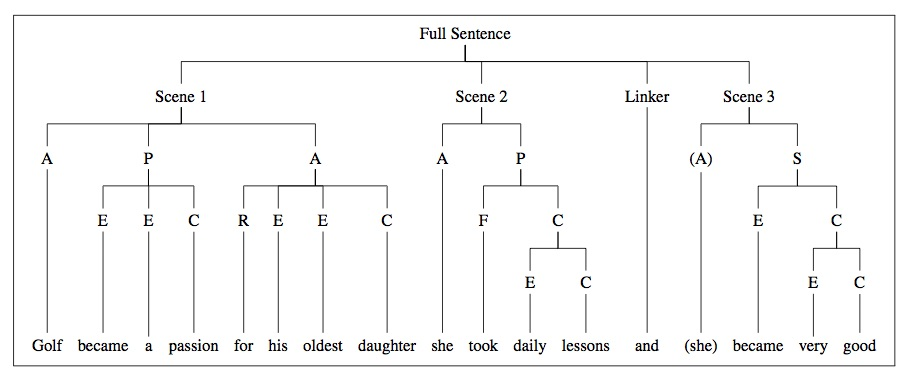
\includegraphics[width=1\textwidth]{ucca-tree}
    \caption{UCCA Tree with scenes}
    \label{ucca-tree}
\end{figure*}

%As you can see 
As can be seen
in Figure~\ref{ucca-tree}, the UCCA annotation results in a tree structure where each leaf is linked to
a word in the sentence at the bottom. A scene must contain a process (P) or a state (S). It can also contain
participants (A) and it can be linked to other scenes by a linker (Linker). Participants, processes and states can be
further analysed into elaborators (E), centres (C) and relators (R). These labels are very 
%high level 
high-level 
and relate to
cognitive concepts which should remain stable across languages.  

The fact that in UCCA
the labels are cognitive concepts and that they are linked directly to words
are both advantages 
when considering which semantic formalism is appropriate for machine translation evaluation.

One of such alternative formalisms is
Abstract Meaning Representation 
%%% Macro broken?
%(AMR; \inparcite{banarescu2013amr}). 
\cite{banarescu2013amr}. 
AMR is being actively developed with 
%the view to 
a view towards
using it as a way of generating 
translations but AMR graphs are not aligned to the words in the sentences. Having more abstract semantic structures 
makes the link between source words, target words, and structures more complex and potentially less useful. 
Furthermore, AMR  has been developed mainly with English in mind, and it remains
to be seen how universal AMR graphs are. See
\shortcite{amr:interlingua:lrec:2014} for first observations of divergences
between English 
%vs.
vs.\ 
Chinese and
Czech AMRs.

Another possible semantic framework for this kind of MT evaluation is Semantic
Role Labelling 
%(SRL; \inparcite{palmer2010semantic}).
\cite{palmer2010semantic}.
SRL has been used in a human translation metric called HMEANT~\cite{lo2011structured}. 
HMEANT uses semantic role labels
to measure how much of the “who, why, when,
where” has been preserved in translation. Annotators are instructed to identify verbs as
heads of semantic frames. Then they attach role
fillers to the heads and finally they align heads
and role fillers in the candidate translation with
those in a reference translation. Using SRL for evaluating SMT has a number of
disadvantages as explored by
\shortcite{birch-EtAl:2013:WMT} for German, \shortcite{bojar:wu:ssst:2012} for
Czech and by \shortcite{chuchunkov-tarelkin-galinskaya:2014:SSST-8} for Russian.
The most important drawbacks are as follows:
\begin{itemize}
\item SRL frames are based around a verb which is particularly problematic for
copular verbs and  when verbs are translated correctly as nouns or correctly
omitted (the verb ``to be'' in some Russian constructions).
\item SRL frames do not cover the entire source sentence and the semantic structure is
therefore not completely defined, importantly links between frames are not
considered and prepositional phrases which attach to nouns are not marked.
\item Even considering a limited set of eleven roles (agent, patient,
experiencer, locative etc.) is problematic because we cannot assume that these roles will 
 remain stable across different languages. 
 When looking at an automatically parsed  English-Chinese  parallel corpora,
 it was shown that 8.7\% of the arguments do not preserve their semantic roles~\cite{fung2006automatic}. 
\end{itemize}

UCCA provides universal semantic structures which 
%has 
have
a minimal set of labels. It provides a complete semantic tree which does not rely on syntactic heads and the semantic structure is grounded directly to the words in the sentence. 
 Even though the set of UCCA labels are fairly restricted,  nevertheless they allow us to determine the most important components of the graph (for example it defines centres and linkers which would be likely to carry more weight than elaborators), and we can use this to better calculate the score. 
We think that UCCA is the
most promising representation for evaluating translation. 

\subsection{Copied from emails}


UCCA-Eval in contrast to HMEANT:

- needs *very* trained UCCA annotators
- we were not very quick at explaining even the Eval annotations, but I guess we could have done better
+ relies only on one structure
+ relies on automatic alignment (in the form of hints only)
  These two positive design decisions are in line with what Dekai observed for HMEANT (see the abstract of http://repository.ust.hk/ir/Record/1783.1-66107): IAA of SRL drops from 90 to 61 when the two aligned structures are from two different annotators.

+ allows for multi-word and even non-contiguous elements
+ allows to indicate the quality of the predicates ("Actions")
+/- expects to cover the whole hypothesis with annotations, whereas HMEANT 'gives up' when the hypothesis is not intelligible, giving a zero score to the bad frame/whole sentence. This can be a good decision for HMEANT, since our way may artificially boost the chances of understanding the sentence.


HMEAN disadvantages:
. Importantly: it disregards copula clauses, nominalizations (which are often translated to verbal clauses), inter-clause relations (discourse markers, complement clauses etc.). UCCA-Eval addresses these.

Actually, I think this is a +/- . UCCA-Eval only needs the semantic evaluation done once for a given test source, whereas for the HMEANT set-up you have to keep annotating MT output. That's a + for UCCA-Eval. However we need bilingual annotators, which should be a -. Of course we could align translation and reference using monolingual annotators, but then we have the problem of alignment.
In the *MEANT papers they mainly test by either
A) correlating the metric to ranking judgements; or
B) using automated versions of the metric for tuning MT systems

I think neither is particularly convincing, but I'm not sure at the moment what we replace them with. Dekai also made a claim about the *MEANT metrics being "interpretable" in the sense that they could guide you towards semantic errors that the MT system may be making, however I don't recall seeing this done in his papers. 


By the claim that HMEANT explains things, Dekai probably means that the score is decomposable, but so is UCCA-Eval and even BLEU. And UCCA-Eval has one benefit over HMEANT: it points to words in the MT output that are aligned with something but do not convey the meaning well (and we know which part of the source meaning). Pure HMEANT might say only that some part of the MT output has no clear frames whatsover (and we do not know which part of the source/reference, unless we add the word alignments).




Differences of our approach:

The annotation experiment that we just conducted differs in two main ways from HMEANT:
1) The semantic framework is different - UCCA vs SRL - and SRL has problems which Omri lists below, some of which Dekai dismissed when they were brought up. Maybe these problems do not matter for MT evaluation or tuning, but I think this would have to be determined empirically.
2) The annotation process is different. We semantically annotate the source, then automatically project it to the translation, and ask bilingual annotators to assess whether this projection shows a good or bad translation. In HMEANT they semantically annotate both the reference and the translation, then align these manually, and assess to what extent they match.

Advatages of our approach:
Here is an additional argument to support the need for target-only intelligibility:
http://www.aclweb.org/anthology/W14-4005
see Table  3 and the text in Section 5.2.
The more frames can people annotate in the hypothesis, the better the hypothesis overall.


\section{Conclusion}

\section*{Acknowledgments}

Do not number the acknowledgment section.
This section should not be presented for the submission version.

\bibliography{main}
\bibliographystyle{acl2016}


\end{document}
